% Concise experimental section; complete records remain in the ABC archive.
\section{Numerical Experiments}
\label{sec:numerical-experiments}

We study outer progress on a W-shaped problem (A), amortized inner calibration
and accuracy restoration (B), and robust RBF
classification on real data (C). The baselines are MCN
\citep{luo2022finding}, GRTR \citep{wang2025gradient}, and, in A, HSDA
\citep{chen2026hsda}. Full trajectories, search results, and diagnostics
are retained in the accompanying experimental archive;
\Cref{app:exp-details} gives the essential reproduction protocol.

\paragraph{Implementation and evaluation.}
We use \emph{parameter-free minimax UTR with persistent SCAR}
(\Cref{alg:gradient-scaled-scar}), abbreviated \emph{Minimax UTR}
in this section. Its standard implementation uses ordinary persistent
SCAR. We denote its early-return variant by \emph{Minimax UTR-early}:
it shares the outer driver but returns from an AR attempt when an
already computed gradient of the original inner objective has halved
the entry residual. Both retain the curvature state and use corrected
oracles. MCN and GRTR use the raw gradient $f_x$ and Schur Hessian
$f_{xx}-f_{xy}f_{yy}^{-1}f_{yx}$. A, C, and the historical B1 controls use $c_0=1/128$;
new B2/B3 use the manuscript's $c_0=2^{-12}$ and fixed $e_1$ secant.
In full UTR runs $\sigma_0=1/\log(e/\epsilon)$, without inputs
$(\ell,\mu,\rho)$ or instance-specific calibration. The historical
settings and early return do not automatically inherit every guarantee
of \Cref{thm:gradient-scaled-scar}; B3 separately audits the native schedule.

We count solved outer subproblems $Q$ and full-vector inner-gradient
queries $N_y$, including initialization and performed residual, secant,
and backtracking checks. UTR's $Q$ includes rejected trials and terminal
validation. Hessian construction, linear algebra, and independent primal
evaluation are separate costs. First hit means the first saved point
meeting the stated true-primal target; function values do not determine
success. Evaluation uses analytic quantities in A and independent
high-accuracy inner solves in B/C, never fed back to the online methods.
Search costs are reported separately. A/C compare configurations tuned
on the same instance, not held-out performance; no statistical or
cross-machine timing advantage is claimed.

\subsection{Benchmark A: outer behavior on a W-shaped problem}
\label{sec:w-shaped}

Following \citet{luo2022finding}, let
\[
 f(x,y)=w(x_3)+x_1y_1-y_1^2/40+x_2y_2-5y_2^2/2,
 \qquad P(x)=10x_1^2+0.1x_2^2+w(x_3),
\]
where, for $r=|t|$,
\[
 w(t)=\begin{cases}
 -0.1r^2+r^3/3,&r\le0.1,\\
 -0.01r+0.001/3,&0.1<r\le0.5,\\
 0.1(r-0.6)^2+(r-0.6)^3/3-2/375,&r>0.5.
 \end{cases}
\]
Here $y^*(x)=(20x_1,x_2/5)$ and $P^*=-2/375$. For the four starts
in \Cref{tab:exp-a-hits}, with $y_0=0$, the common target is
\begin{equation}
 \|\nabla P(x)\|\le10^{-8},\qquad
 \lambda_{\min}(\nabla^2P(x))\ge-\sqrt{2\cdot10^{-8}}.
 \label{eq:wshape-target}
\end{equation}
Each baseline is tuned separately at each start, minimizing
$(Q^{\rm hit},N_y^{\rm hit})$ with a fixed tie order and 100-update
budget. MCN/HSDA use 800/8,000 configurations per start; GRTR uses a
staged search. Minimax UTR retains native stopping with a 2,000-subproblem
safety budget. These are not equal-search-budget comparisons
(\Cref{app:exp-a}).

\begin{table}[tb]
\centering\small
\setlength{\tabcolsep}{4pt}
\begin{tabular}{lccccc}
\toprule
$x_0$ & MCN & GRTR & HSDA & \shortstack{Minimax\\UTR} & \shortstack{Minimax\\UTR-early}\\
\midrule
$(.001,.001,.001)$ & $11/440$ & $15/300$ & $11/440$ & $11/23{,}784$ & $11/1{,}528$\\
$(0,0,1)$ & $6/24$ & $6/30$ & $7/28$ & $6/8$ & $6/8$\\
$(.1,.1,.1)$ & $14/560$ & $20/400$ & $14/560$ & $9/19{,}525$ & $9/1{,}326$\\
$(1,.1,.1)$ & $16/640$ & $23/460$ & $17/680$ & $9/18{,}203$ & $9/1{,}389$\\
\bottomrule
\end{tabular}
\caption{A: $Q^{\rm hit}/N_y^{\rm hit}$, including initialization.
Baseline parameters are selected separately for each row; UTR settings
are fixed. These are first-hit, not native-termination, costs.}
\label{tab:exp-a-hits}
\end{table}

Both UTR variants match the smallest reported outer count at the first
two starts and improve it at the other two. Their outer trajectories
coincide, while early return sharply reduces full-SCAR work
(\Cref{fig:wshape-benchmark}). Tuned baselines nevertheless use fewer
inner queries at three starts. The quadratic inner makes the corrected
value and gradient exact in exact arithmetic, so A tests outer behavior,
not nonlinear tracking. Also, the cubic tails preclude a finite global
joint gradient-Lipschitz constant; this literature benchmark does not
verify every assumption of the minimax theorem.

\begin{figure}[tbp]
\centering
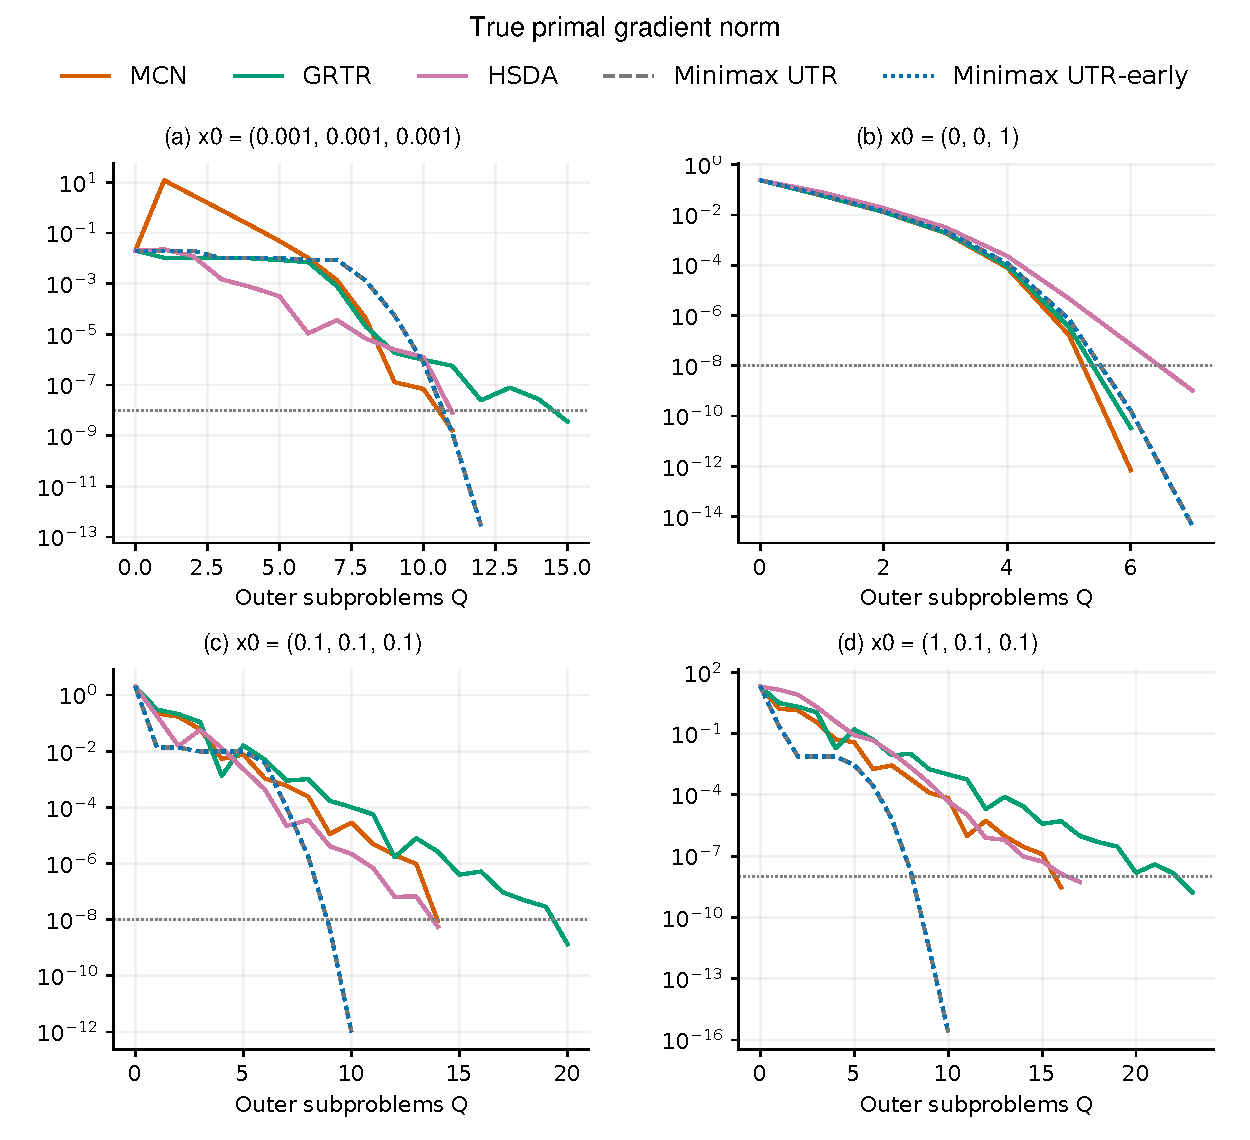
\includegraphics[width=0.90\linewidth]{figures/experiments/A_stationarity.pdf}
\caption{A: true gradient norm versus $Q$ at all four starts.
Baselines end at first hit; UTR retains native termination. Full/early
UTR overlap. Actual nonmonotonicity is retained; no running minimum.}
\label{fig:wshape-benchmark}
\end{figure}

\subsection{Benchmark B: amortized inner work}
\label{sec:exp-b}

For $x=(u,v)$, define the curved-valley payoff
\begin{align}
 P_0(u,v)&=\sqrt{1+(u-35)^2}-1+0.35[1-\cos(0.7(u-35))]
                 +\log\cosh(v-h(u)),\nonumber\\
 h(u)&=0.8\sin(u/2)+0.4\sin(\sqrt2u/2),\qquad
 C=2^{-1/2}\begin{pmatrix}1&1\\1&-1\end{pmatrix},\nonumber\\
 f_D(x,y)&=P_0(x)+0.1\sum_{i=1}^2[1-\cos((Cx)_i+d_i y_i)]
                    -3\|Dy\|^2,
 \label{eq:exp-b-payoff}
\end{align}
where $D=\operatorname{diag}(d_1,d_2)$ is invertible. The base instance
uses $D=I$, $x_0=y_0=0$, $\epsilon=10^{-6}$, and bounds
$(\ell,\mu,L_y,\rho,\bar M_P)=(6.2,5.9,6.1,4.32283,4.14516)$.
The nonlinear inner maximizer satisfies
$0.1\sin((Cx)_i+z_i^*)=6z_i^*$ for $z=Dy$; hence $|z_i^*|\le1/60$.
Online derivatives require no root solve. Roots are used only for
exact-primal controls and offline evaluation; $P\ne P_0$ and $P^*$ is
not assumed known.

Oracle-error scaling, exact-path reproduction, and exact-MCN
outer-scale controls are retained as auxiliary checks in
\Cref{app:exp-b-controls}; they do not isolate the source of tracking savings.

\paragraph{B1: reusing curvature calibration.}
Freeze exact UTR's 47 accepted points and incoming scales $\sigma_t$.
For $D_\gamma=\operatorname{diag}(\gamma^{-1/2},\gamma^{1/2})$,
$\gamma\in\{1,2,4,8\}$, the primal is unchanged. Recount all work from
zero and require the same intrinsic target at every point:
\begin{equation}
 \|D_\gamma^{-1}\nabla_yf_{D_\gamma}(x_t,y_t)\|\le r_t,
 \qquad r_t=\frac{c_0\ell\sqrt\epsilon}{4\sigma_t}.
 \label{eq:exp-b-intrinsic}
\end{equation}
The external scheduler knows $\ell$; SCAR does not. Solvers update in
$y$, without preconditioning, and AGD receives
$L_{y,\gamma}=6.1\gamma$, $\mu_\gamma=5.9/\gamma$.
Persistent SCAR-early retains $y,\nu,\mathcal M$; warm restart retains
only $y$; cold restart resets both. All checks and secants are charged.

\begin{table}[tb]
\centering\small
\setlength{\tabcolsep}{4.5pt}
\begin{tabular}{rrrrrrr}
\toprule
$\gamma$ & $\bar\kappa_y$ & Persistent & Warm restart & Cold restart & Warm AGD & Cold AGD\\
\midrule
1 & 1.03 & 462 & 391 & 445 & 195 & 187\\
2 & 4.14 & 632 & 679 & 787 & 1,068 & 1,255\\
4 & 16.54 & 1,439 & 5,837 & 6,316 & 2,566 & 3,017\\
8 & 66.17 & 3,654 & 17,297 & 18,325 & 5,492 & 6,439\\
\bottomrule
\end{tabular}
\caption{B1: fixed-path $N_y^{\rm path}$ at identical intrinsic targets.
The three restart columns use SCAR-early; AGD knows the analytic
conditioning bounds. The primal and outer path are unchanged.}
\label{tab:exp-b-conditioning}
\end{table}

At $\gamma=1$, persistent full SCAR costs 17,021 queries versus 462
for early, a factor of 36.84. AGD is still cheaper, and persistence
itself costs more than warm restart. At $\gamma=8$, persistence instead
saves a factor of 4.73 over warm restart. Downward curvature corrections
$\nu\leftarrow\nu/4$ number 2/89/92 for persistent/warm/cold restart
(1/44/46 at $\gamma=4$). Only 46 of the 13,643 saved queries at
$\gamma=8$ are secant savings; the rest includes all halving and checking
work, not solely curvature identification. All 940 returned points
satisfy the common target. This supports reuse of curvature calibration, not removal of an
accuracy logarithm or uniform superiority to AGD. Replay excludes rejected trials and outer validation, so 462
and the full-run cost 779 are distinct quantities.

\paragraph{B2: restoring accuracy under joint refinement.}
To separate warm starts from resetting curvature, fix $D=\mathrm{diag}(1/2,2)$
and subdivide each of the same 46 path segments into
$m\in\{1,2,4,8,16,32\}$ equal pieces. There are $T_m=46m+1$
requests, with $\epsilon_m=10^{-3}/m^2$ and the common native target
\[
 \|f_y\|\le\tau_m=\frac{c_0(24.5)\sqrt{\epsilon_m}}{4\bar\sigma}
       =\frac{1.7514703\times10^{-4}}{m},\qquad
 \bar\sigma=0.26998732,\quad c_0=2^{-12}.
\]
Warm-PSCAR carries $y$ forward; Cold-PSCAR starts each request at zero.
\emph{Both retain their own curvature states and use ordinary SCAR,
with early return disabled}. Warm/cold AGD use the same fixed
$(L_y,\mu_y)=(24.4,1.475)$ and reset momentum each request.
Each method and mesh starts with a fresh state. These are artificial
moving-target requests, not native UTR iterations.

Since $\|f_y(x',y)-f_y(x,y)\|\le.2\|x'-x\|$, warm starts satisfy
$R_{\rm in}/\tau_m\le1+.2\|X_{j+1}-X_j\|/\tau_{\rm ref}$,
independent of $m$. At a fixed nonzero cold residual the ratio instead
grows as $m$. We report this entry burden alongside actual queries
(\Cref{fig:exp-b-restoration}), rather than interpreting the sufficient
budget $\lceil\log_2(R_{\rm in}/\tau_m)\rceil_+$ as an observed count
or a lower bound.
From $m=1$ to 16, queries per request change from $859$ to $883$
for Warm-PSCAR and $1{,}012$ to $1{,}485$ for Cold-PSCAR;
AGD changes from $39.3$ to $40.7$ and $48.8$ to $69.9$, respectively.
Neither PSCAR arm makes a downward-$\nu$ correction.
This separates accuracy restoration from repeated initialization of curvature;
ordinary SCAR remains much more expensive than known-bound AGD.
At $m=32$, Warm-PSCAR uses $890$ queries per request; Cold-PSCAR
completes only $1299/1473$ requests within the frozen $2\times10^6$-query
budget and is excluded from full-path averages.

\begin{figure}[tb]
\centering
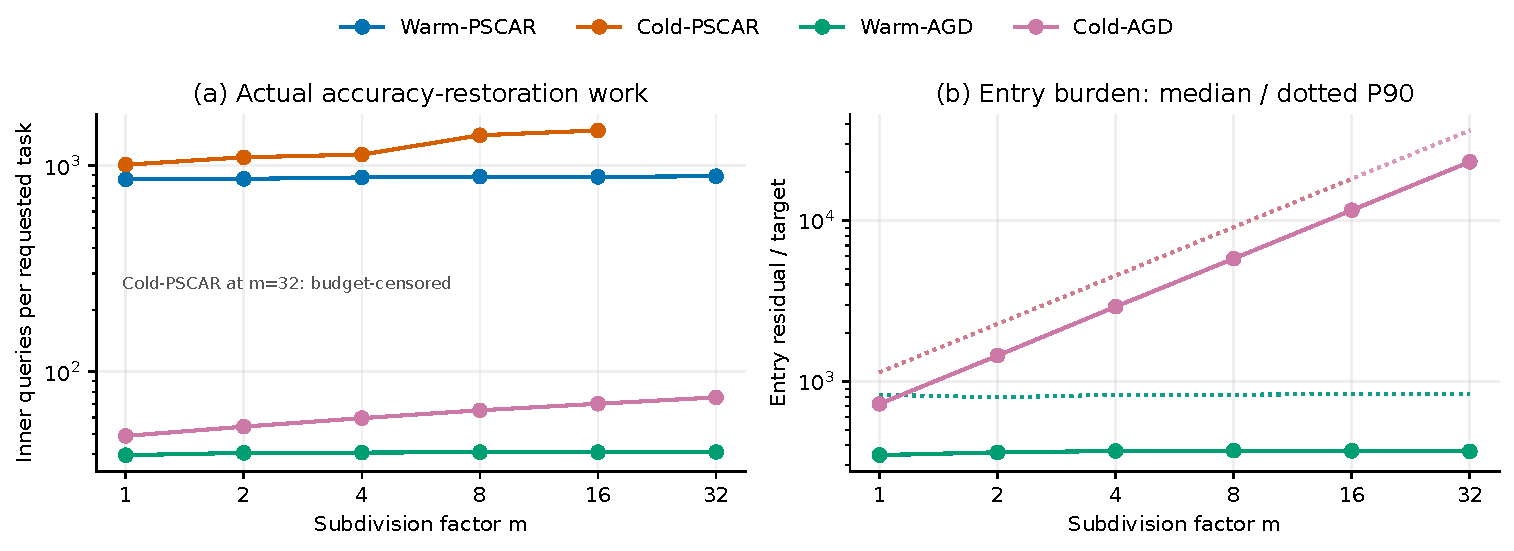
\includegraphics[width=\linewidth]{figures/experiments/B_accuracy_restoration.pdf}
\caption{B2: actual average work and relative entry residual under joint
path/accuracy refinement. Solid curves in the right panel are medians;
dotted curves are 90th percentiles. Both PSCAR arms retain curvature
state. Only complete paths enter the average-cost curves; cold entry residuals
coincide by construction.}
\label{fig:exp-b-restoration}
\end{figure}

\paragraph{B3: work along the native algorithm.}
Finally, run \Cref{alg:gradient-scaled-scar} on the same $D$, from zero,
for $\epsilon=10^{-3},\ldots,10^{-7}$, using ordinary SCAR,
$c_0=2^{-12}$, the prescribed fixed halving counts, and native validation.
A float64 trial reached its residual floor before completing its scheduled
halvings; we retain that failure and use 100-digit arithmetic for this
five-run audit, without replacing the schedule by early or target stopping.
All five 100-digit runs terminate and pass independent gradient checks,
using $215{,}781$, $189{,}531$, $173{,}125$, $308{,}127$, and $292{,}759$
queries, respectively. Accepted-trial tracking accounts for $94.9$--$97.5\%$.
These full-SCAR costs are distinct from early-return costs; changing
$\sigma_0$ with $\epsilon$ also changes the realized outer path.
We partition every query into initialization, accepted/rejected trials,
refresh, failed validation, terminal trial, or successful validation.
For ordinary accepted steps, the recorded counts satisfy
$S_{\rm tr}\le16K+\epsilon^{-3/2}C_3$, where
$C_3=\sum\sigma_k^3\|d_k\|^3$; normal returns also satisfy $Q=K+J+1$.
These are implementation/accounting checks, not evidence that the bound
is tight or that five precision settings establish a complexity rate.

\subsection{Benchmark C: robust RBF classification}
\label{sec:exp-c}

We use WDBC's 569 samples and 30 features, with a seed-2026 stratified
split into 455 training and 114 test samples. Standardization is fitted
only on training data; test labels are not used for selection.
With five trainable centers $u_j\in\mathbb R^{30}$, let
\[
 s_x(a)=\sum_{j=1}^5\tanh(v_j)e^{-\|a-u_j\|^2/8}+\tanh(v_0),
 \qquad x\in\mathbb R^{156}.
\]
For labels $b_i\in\{-1,1\}$ and unconstrained sample-wise perturbations
$z_i=\sqrt n\,y_i$, $n=455$, we minimize the maximum over
$y\in\mathbb R^{455\times30}$ of
\begin{equation}
 f(x,y)=\frac1n\sum_{i=1}^n
 \left[\log(1+e^{-b_i s_x(a_i+\sqrt n\,y_i)})
                  -\|\sqrt n\,y_i\|^2\right]
                  +\frac{10^{-4}}2\|x\|^2.
 \label{eq:exp-c-payoff}
\end{equation}
The bandwidth and adversarial penalty are fixed at 2. Separability
requires only $30\times30$ inner blocks and a $156\times156$ Schur
Hessian. All methods use $y_0=0$ and the same frozen negative-curvature
start, selected geometrically from 33 predetermined candidates, without
algorithm outcomes: initially $P=.8783993$, $\|\nabla P\|=.1371588$,
and $\lambda_{\min}=-.1574913$ (\Cref{app:exp-c-initialization}).

\paragraph{Practical calibration.}
Both baselines use warm-start AGD with restarted momentum,
$L_y=3.25$, $\mu_y=.175188$, step $1/L_y$, and momentum
$(\sqrt{L_y/\mu_y}-1)/(\sqrt{L_y/\mu_y}+1)$. We search
\begin{equation}
\begin{aligned}
 M&\in\{10^{-4},10^{-3},10^{-2},10^{-1},1,10\} &&\text{(MCN)},\\
 \widetilde L_2&\in\{10^{-4},10^{-3},10^{-2},10^{-1},1\} &&\text{(GRTR)},\\
 \tau_{\rm inner}&\in\{10^{-10},10^{-8},10^{-6},10^{-4},10^{-2}\}
                                                       &&\text{(both)}.
\end{aligned}
\label{eq:exp-c-grid}
\end{equation}
Inner stopping requires $\|\nabla_y f\|\le\tau_{\rm inner}$ in the
normalized coordinates. MCN uses cubic coefficient $M/6$. GRTR sets
$\sigma_{\rm reg}=\sqrt{\widetilde L_2}/2$ and
$r=1/(4\sqrt{\widetilde L_2})$. Its radius is
$r\sqrt{\max\{\|g_{\rm raw}\|,\epsilon\}}$; the Hessian shift is
$\sigma_{\rm reg}\sqrt{\|g_{\rm raw}\|}I$.
These practical tolerances do not carry the original oracle-error
certificates. Each of 55 configurations has budgets $Q\le10^4$,
$N_y\le10^6$, and 900 online seconds. Selection minimizes
$(N_y^{\rm hit},Q^{\rm hit})$ with fixed tie order, using only the true
gradient target $10^{-6}$. Native flags do not certify external success;
independent evaluation and stagnation handling are specified in
\Cref{app:exp-c-stopping}.

\begin{table}[tb]
\centering\small
\setlength{\tabcolsep}{5pt}
\begin{tabular}{llrrr}
\toprule
Method & Configuration & $Q^{\rm hit}$ & $N_y^{\rm hit}$ & $\|\nabla P\|_{\rm hit}$\\
\midrule
Minimax UTR-early & Fixed & 154 & 1,186 & $3.19\cdot10^{-7}$\\
MCN & $M=10^{-3},\ \tau=10^{-4}$ & 93 & 563 & $9.06\cdot10^{-8}$\\
GRTR & $\widetilde L_2=10^{-4},\ \tau=10^{-4}$ & 30 & 356 & $9.26\cdot10^{-7}$\\
\bottomrule
\end{tabular}
\caption{C: initialization-inclusive first-hit costs. Baselines are
selected on this same instance. All hit values satisfy
$P\approx.493433306$, $\lambda_{\min}\approx6.48\cdot10^{-4}$;
this does not certify global optimality. Search costs are separate.}
\label{tab:exp-c-hits}
\end{table}

The selected MCN/GRTR use 52.5\%/70.0\% fewer queries than fixed
Minimax UTR-early (\Cref{tab:exp-c-hits}), and neither selected baseline
rebounds above $10^{-6}$ after first hit. MCN nevertheless first raises
$P$ to 5.6712 (\Cref{fig:exp-c-trajectories}). Of the practical grids,
20/30 MCN and 18/25 GRTR settings hit; all $\tau=10^{-2}$ settings miss.
For GRTR at $\widetilde L_2=.01$, tightening $\tau$ from $10^{-4}$ to
$10^{-10}$ leaves $Q^{\rm hit}=229$ but raises queries from 1,073 to
10,523. More inner accuracy need not improve outer progress.

\begin{figure}[tb]
\centering
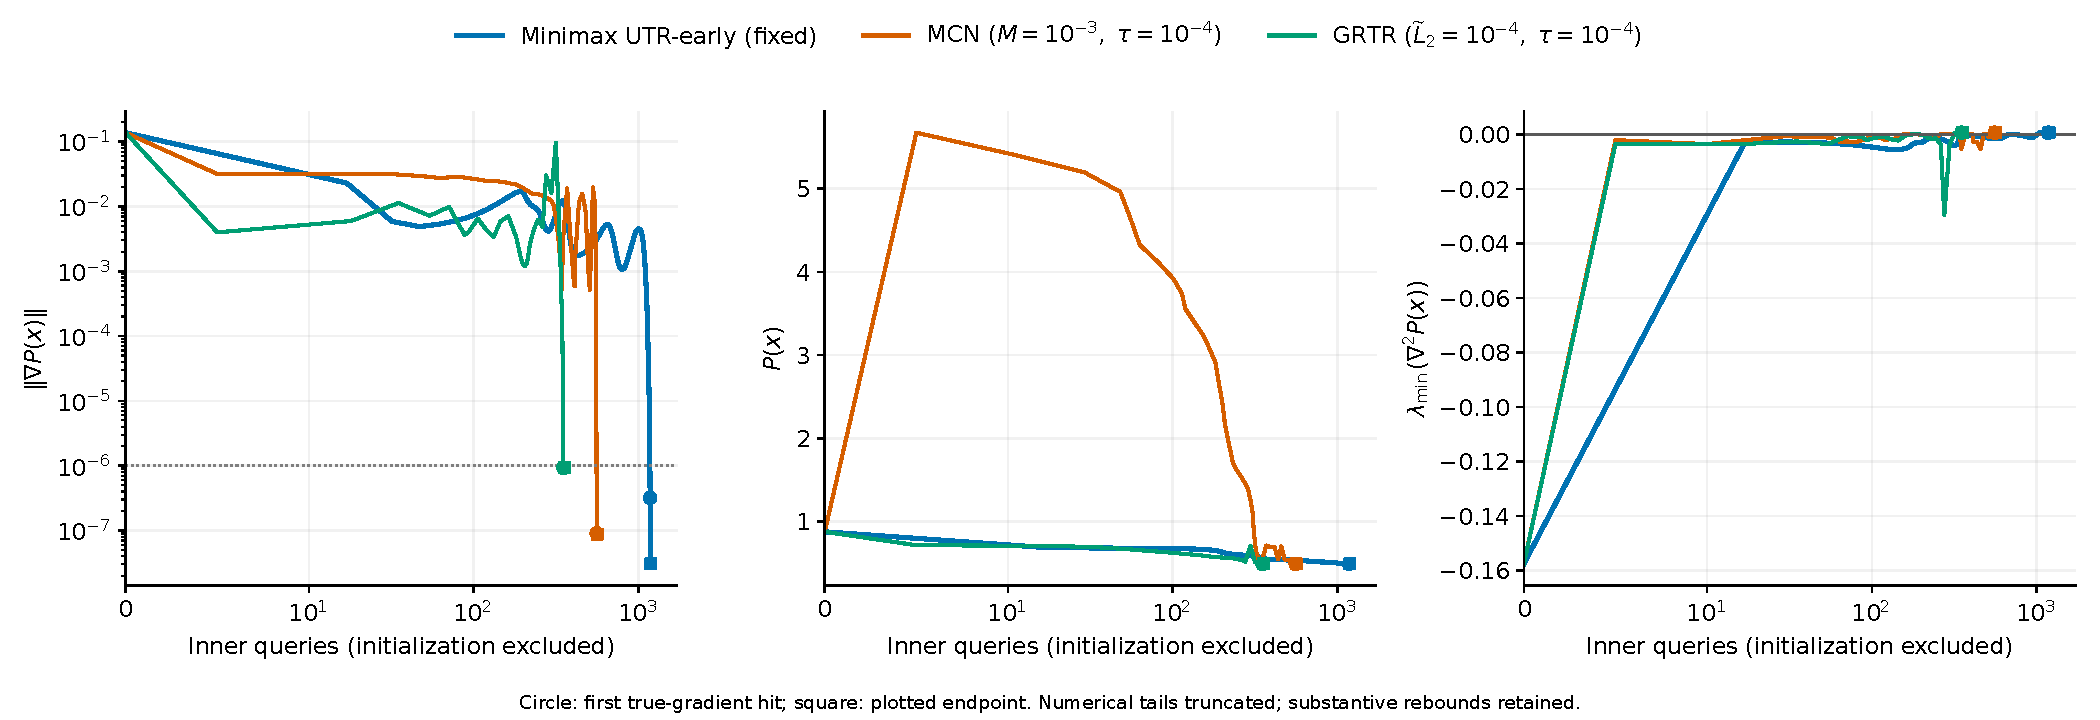
\includegraphics[width=\linewidth]{figures/experiments/C_best_three.pdf}
\caption{C: true gradient, objective, and minimum Hessian eigenvalue.
Plots subtract initialization (10 queries for UTR, 6 per baseline);
tables include it. Circles denote first hit, squares display endpoints.
The symmetric-log axis retains zero. Only terminal numerical tails are
trimmed; actual rebounds remain (\Cref{app:exp-c-stopping}).}
\label{fig:exp-c-trajectories}
\end{figure}

Formula-scale MCN/GRTR references with $M\approx1.0373\cdot10^7$ and
$L_2\approx2.0281\cdot10^6$ still have gradient norms .01485/.17086
after 10,000 subproblems. They also use different inner dynamics and
formula-derived tolerances; this contrast is not solely an outer-scale
effect. The supplied joint $\rho=73.10$ was not independently globally
certified (\Cref{app:exp-c-reference}).

Together, A demonstrates outer progress, B identifies inner-work
mechanisms and their limits, and C shows the competitiveness of
instance-tuned fixed-scale methods. We do not infer uniform empirical
dominance, transfer of selected parameters to unseen starts, or improved
test accuracy from these optimization experiments.
